%!TEX root = ../../main.tex

\chapter{Approach}
\label{chap:appr}

This chapter describes how the benchmarking was approached in this work. It also describes what data was generated how to facilitate the benchmarks in a repeatable manner.

%The result of the data generation that was used for these benchmarks can be found under \url{https://github.com/josias-mueller/letztestudienarbeit_data}.
% github limits filesize to 100mb :c

\section{Variables}

The concept of benchmarking rests on determinism: The expectation that if none of the input variables of a process change, the output remains the same - no matter how many times it is executed. If this is not the case, that means that one or more variables have been overlooked. The intention is to learn all variables relevant to the output of a process, learn how exactly they modify the output as to be able to manipulate them to create a favorable change in the output.

% Benchmarking is heavily focussed around variables: Unknown and uncontrolled variables break benchmarks, make them unreliable. Thus careful consideration and handling of variables is necessary. Benchmarking is easier the fewer variables are at play - this is why as many variables as sensibly possible are eliminated. More on the elimination of variables can be found in \autoref{sec:considerations}.

% One variable that will be investigated in these benchmarks is the size
% Various datasets were used in the benchmarks. In abstraction, every dataset could be viewed as a combination of two additional variables: element count and element distribution.

During benchmarking all variations of a predetermined set of each of the following variables are tested, except for those that cannot be executed, e.g. because of memory constraints:

\subsection{Element Size}

Varying the size of the indexed elements themselves primarily affects the memory consumption. If the size of the elements is increased, this increases the theoretical minimum of memory needed to store the data. However, since transferring more data takes more time the expectation is that everything will slow down as the element size increases. In addition to this, increasing the size per element also means that fewer elements fit in a \textit{cache\footnote{As memory size increases, it becomes slower - cache refers to a secondary part of memory, that is smaller and thus faster.} line}\footnote{A cache line is the smallest unit of memory that can be mapped to the \acsp{CPU}'s internal cache}.

There are 5 different element sizes used in the benchmarks:

\begin{itemize}
    \item Element: 12 Bytes (latitude and longitude as floats and a 32 bit id)
    \item BiggerElement: 24 Bytes (latitude and longitude as floats and 128 bits of data)
    \item BigElement: 256 Bytes (latitude and longitude as floats and 31 64 bit data fields)
    \item VeryBigElement: 512 Bytes (latitude and longitude as floats and 63 64 bit data fields)
    \item VeryVeryBigElement: 1024 Bytes (latitude and longitude as floats and 127 64 bit data fields)
\end{itemize}

\subsection{Element Count}

Varying the number of elements in the index has a similar effect as varying the size in that the theoretical minimum of memory needed to store the data is increased. However, the number of elements that fit in a cache line stays the same. The smallest used dataset consists of 16,200 elements where the largest contains 4,147,200 elements. The expectation is that everything will slow down as more and more elements are added to the index.

\subsection{Element Distribution}

Varying element distribution is not quite as simple as varying the element size or the number of elements as it is not just a number. Inspecting how the indices behave with different distributions is interesting as this information could be used to pick the best index based on the distribution of the data - should the results prove significant.


\subsection{Datasets}

In abstraction, every dataset could be viewed as a combination of two additional variables: element count and element distribution.

\subsubsection{Data Origins}

\paragraph{Real} Real data, as in data points extracted from physical reality are interesting because they are the most obvious application for indices as described in this work.

\paragraph{Synthetic} Synthetic data is convenient as it can just be generated. However, a system under synthetic load (or using synthetic data in general) may very well not behave the same way it would under a real load (or with real data respectively).

To create a better understanding of the used datasets there will be visualisations showing every datapoint on a map, this visualisation is created by serialising all of the datapoints in a dataset as GeoJSON (refer to \autoref{subs:geojson}) and loading all of this data with Leaflet (refer to \autoref{subs:leaflet}). In addition to this, to provide a frame of reference, in all of these visualisations a GeoJSON dataset\cite{countryjson} that outlines all countries on earth is displayed beneath the actual dataset.

\subsubsection{Synthetic - Symmetric}

The generated \textit{Symmetric} dataset is constructed as follows:

\begin{lstlisting}[label=lst:orderedgen,caption={[Generation of the coordinates  for the symmetric dataset.]Generation of the coordinates  for the symmetric dataset.}]
    for every multiplier in [1, 4, 16, 64, 256]
        generate all combinations where
            x(*@ \(\in\) @*)[-180; 180), step =(*@ \(\frac{2}{\sqrt{multiplier}}\) @*)
            and
            y(*@ \(\in\) @*)[-90; 90), step =(*@ \(\frac{2}{\sqrt{multiplier}}\) @*)
\end{lstlisting}

This results in \(multiplier*180*90\) points per dataset:

\begin{table}[H]
    \begin{tabular}{l|l|l|l|l|l}
        Multiplier         & 1      & 4      & 16      & 64        & 256       \\ \hline
        Number of elements & 16,200 & 64,800 & 259,200 & 1,036,800 & 4,147,200
    \end{tabular}
    \caption[Number of elements in each symmertic dataset.]{Number of elements in each symmertic dataset.}
    \label{tab:symcount}
\end{table}

When drawn on a map these datasets may look as shown in \autoref{fig:ordered}\footnote{Fun fact: \autoref{fig:ordered256} took Leaflet about half an hour and 80 GB of memory to render - that was surely worth it, right?}.

\begin{figure}[H]
    \centering
    \begin{subfigure}{0.458\textwidth}
        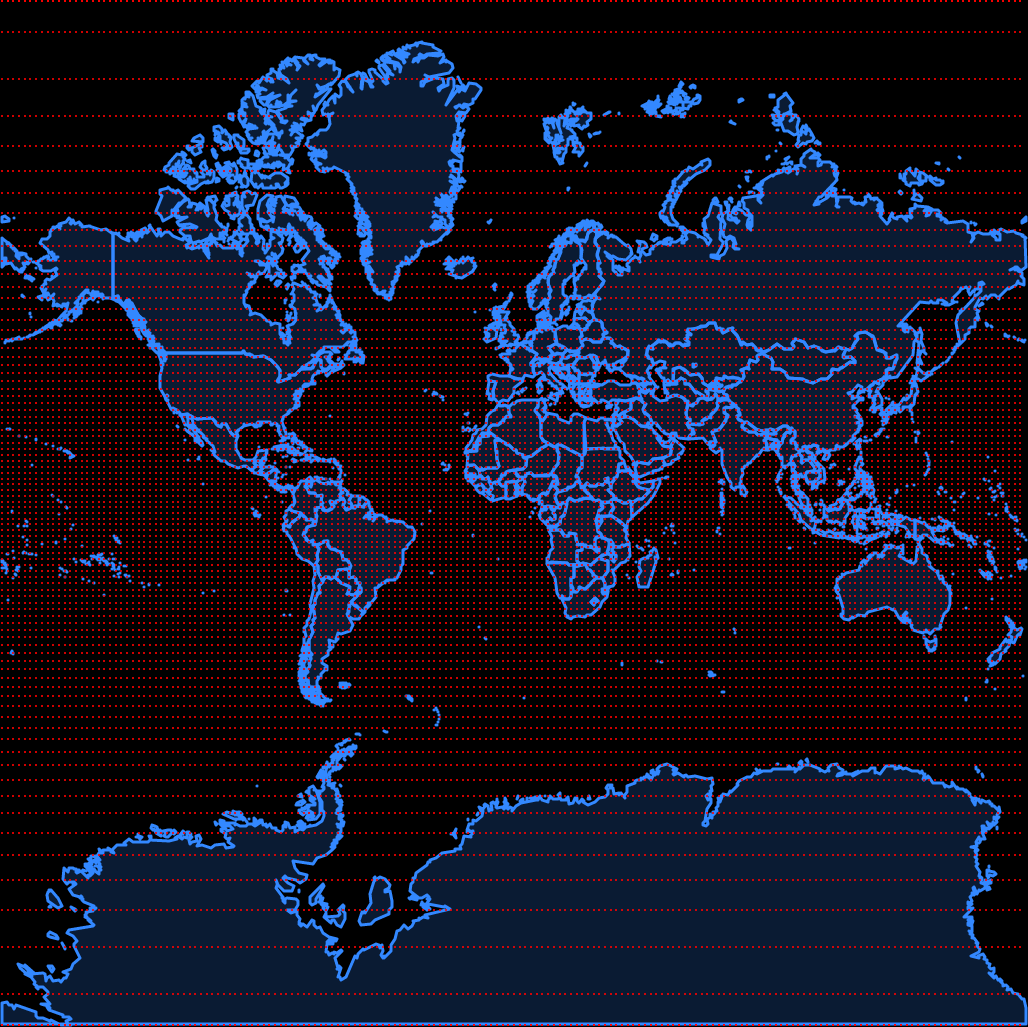
\includegraphics[width=\textwidth]{ordered1}
        \caption[Symmetric dataset with multiplier 1.]{Symmetric dataset with multiplier 1.}
        \label{fig:ordered1}
    \end{subfigure}
    \hfill
    \begin{subfigure}{0.458\textwidth}
        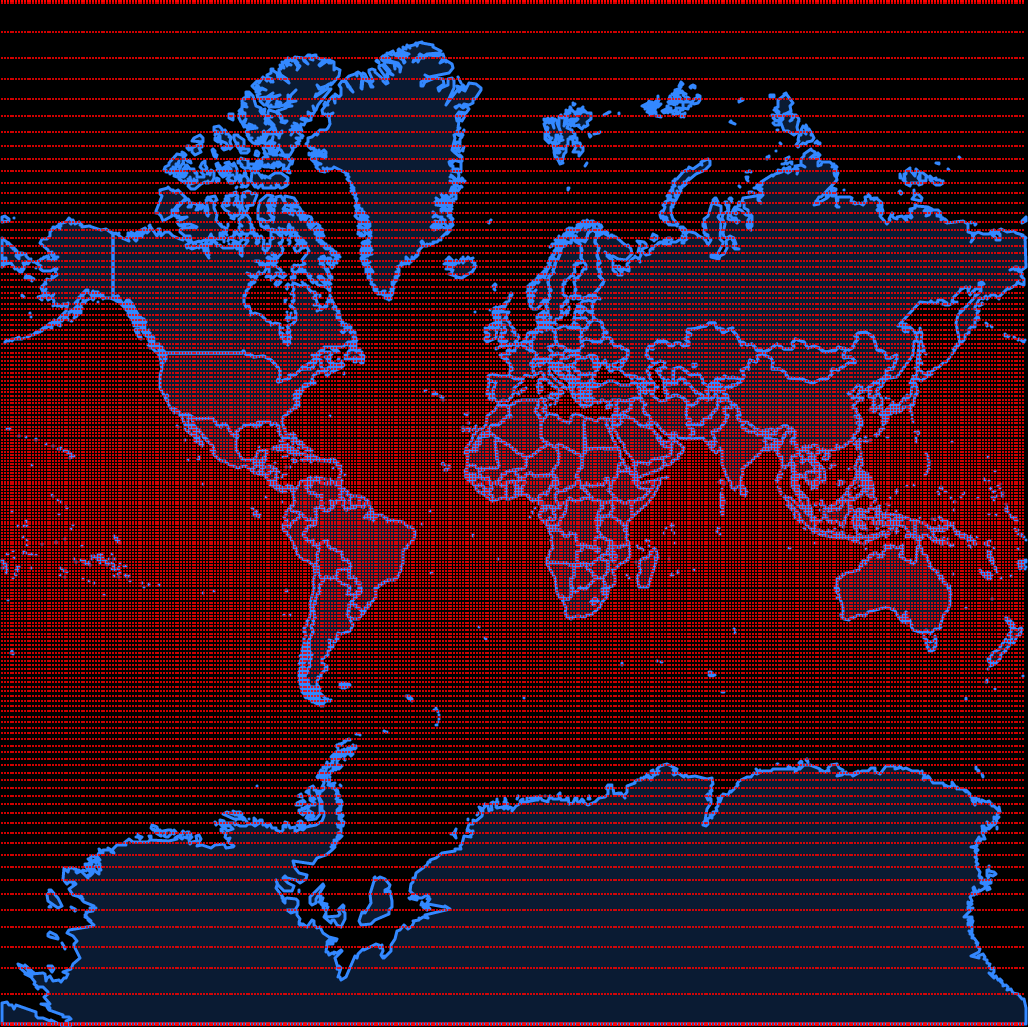
\includegraphics[width=\textwidth]{ordered4}
        \caption[Symmetric dataset with multiplier 4.]{Symmetric dataset with multiplier 4.}
        \label{fig:ordered4}
    \end{subfigure}
    \hfill
    \begin{subfigure}{0.458\textwidth}
        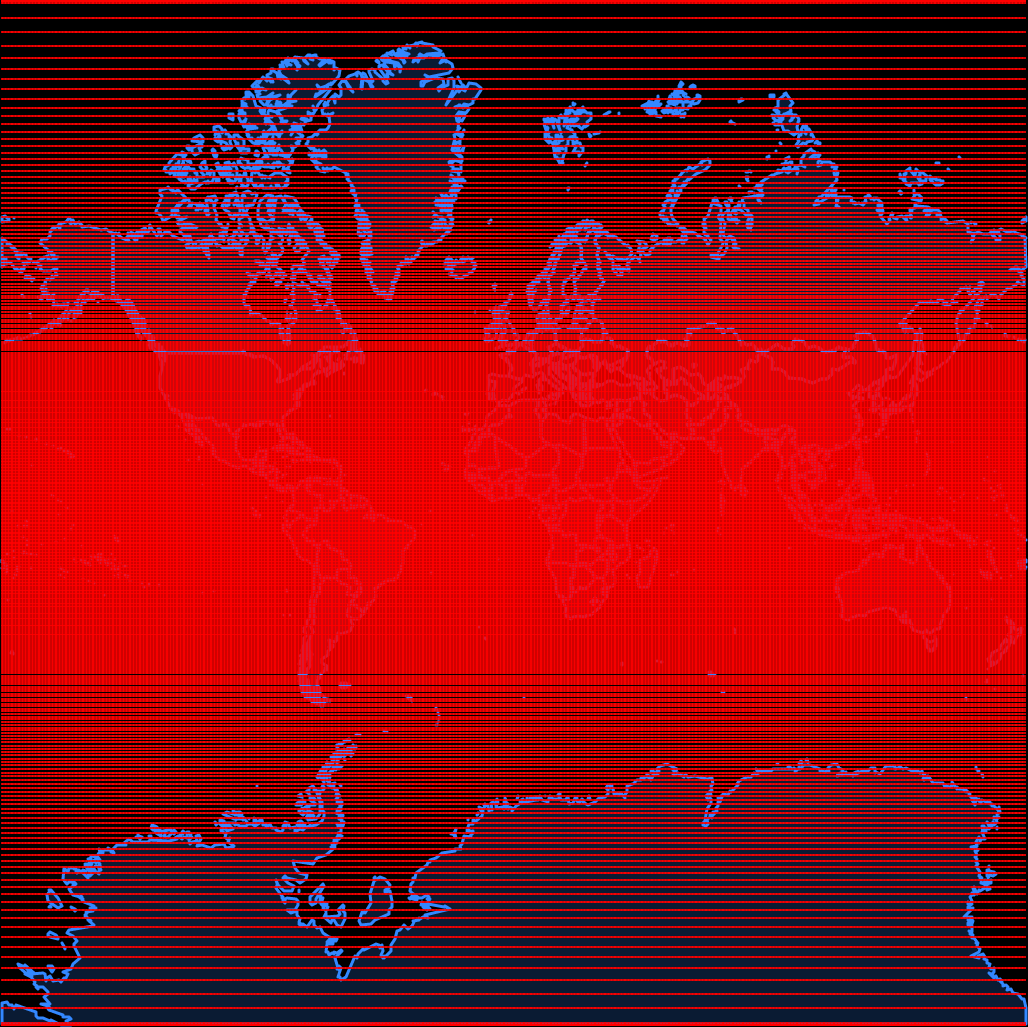
\includegraphics[width=\textwidth]{ordered16}
        \caption[Symmetric dataset with multiplier 16.]{Symmetric dataset with multiplier 16.}
        \label{fig:ordered16}
    \end{subfigure}\hfill
    \begin{subfigure}{0.458\textwidth}
        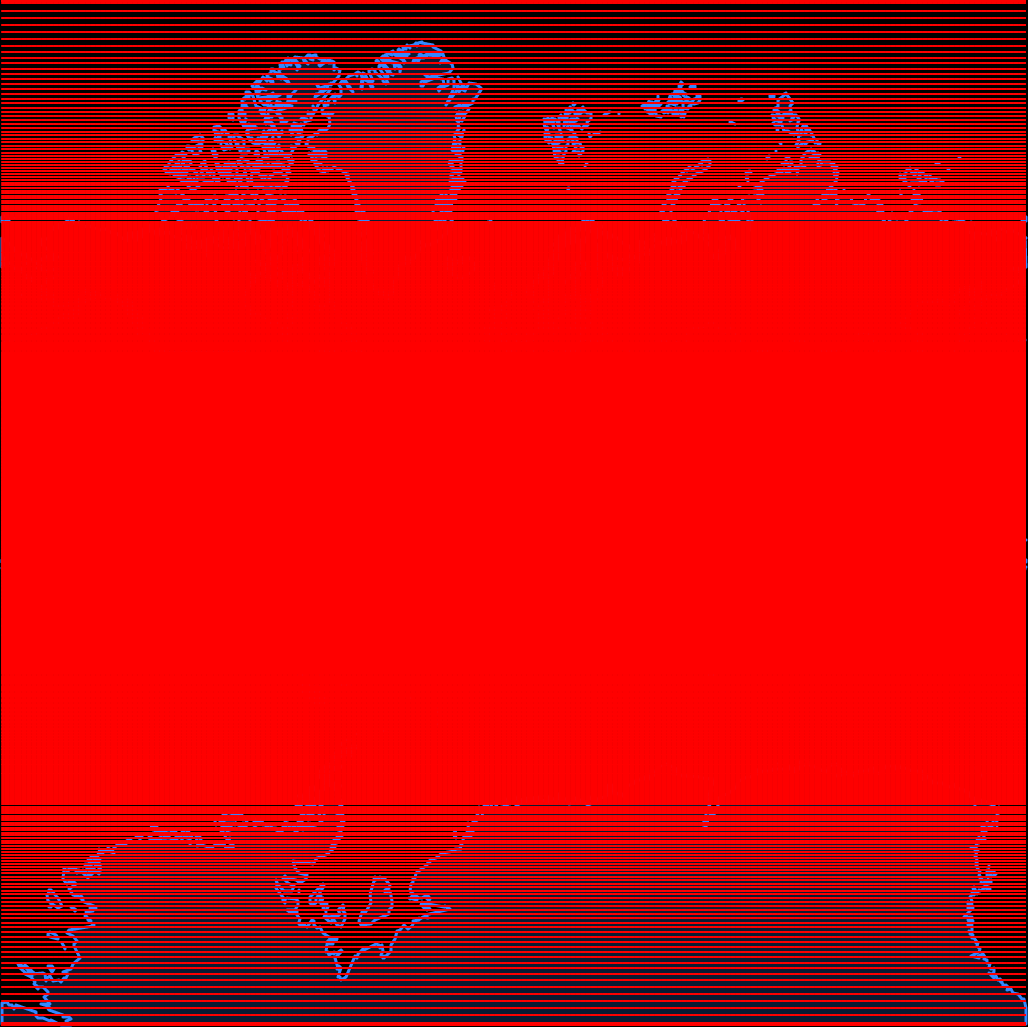
\includegraphics[width=\textwidth]{ordered64}
        \caption[Symmetric dataset with multiplier 64.]{Symmetric dataset with multiplier 64.}
        \label{fig:ordered64}
    \end{subfigure}\hfill
    \begin{subfigure}{0.458\textwidth}
        
\includegraphics[width=\textwidth]{ordered256}
        \caption[Symmetric dataset with multiplier 256.]{Symmetric dataset with multiplier 256.}
        \label{fig:ordered256}
    \end{subfigure}
    \caption[All symmetric datasets.]{All symmetric datasets.}
    \label{fig:ordered}  
\end{figure}

\subsubsection{Synthetic - Random}
\label{subsubs:random}

This dataset is constructed completely randomly via a uniform distribution - no limitations besides the ones already defined in \autoref{lst:orderedgen}. Since the intention with this dataset is to determine whether element distribution affects performance, the other variable - in this case element count should be eliminated. To achieve this, the number of elements in this dataset is derived from the element count of the other datasets. To reduce the chances of accidentally generating a dataset that favours one implementation over the other, this dataset has been generated and tested multiple times for each element count. The expectation with this is that there are no significant differences in the results of the datasets generated with the same parameters. The complete list of element counts is as follows in \autoref{lst:synthcounts}:

\begin{lstlisting}[label=lst:synthcounts,caption={[Element counts of the synthetic datasets.]Element counts of the synthetic datasets.}]
    16,200, 44,692, 64,800, 140,974, 259,200, 1,036,800, 3,808,651, 4,147,200
\end{lstlisting}

\begin{figure}[H]
    \centering
    \begin{subfigure}{0.4\textwidth}
        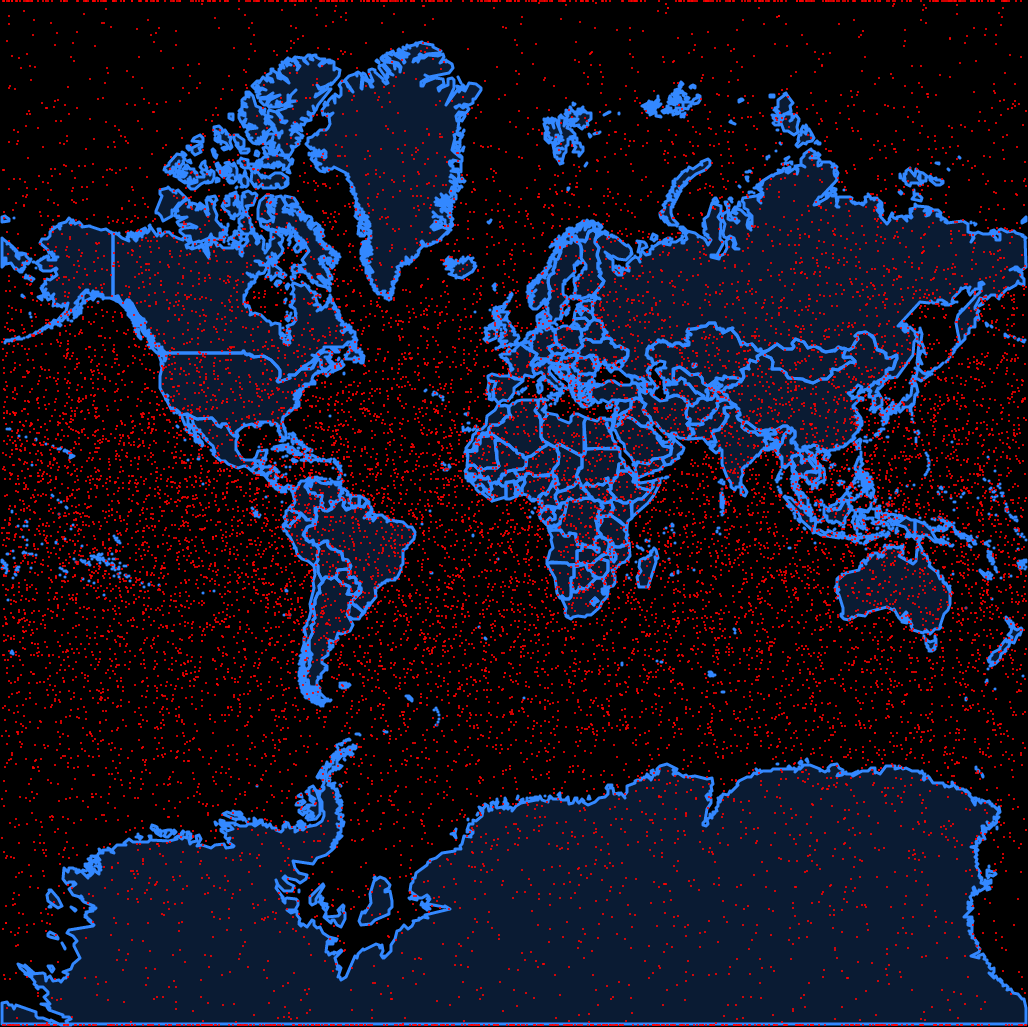
\includegraphics[width=\textwidth]{uniform/16200_0}
        \caption[The first of three purely random datasets with an element count of 16200.]{The first of three random datasets with an element count of 16200.}
        \label{sfig:uniform16200_0}
    \end{subfigure}\hfill
    \begin{subfigure}{0.4\textwidth}
        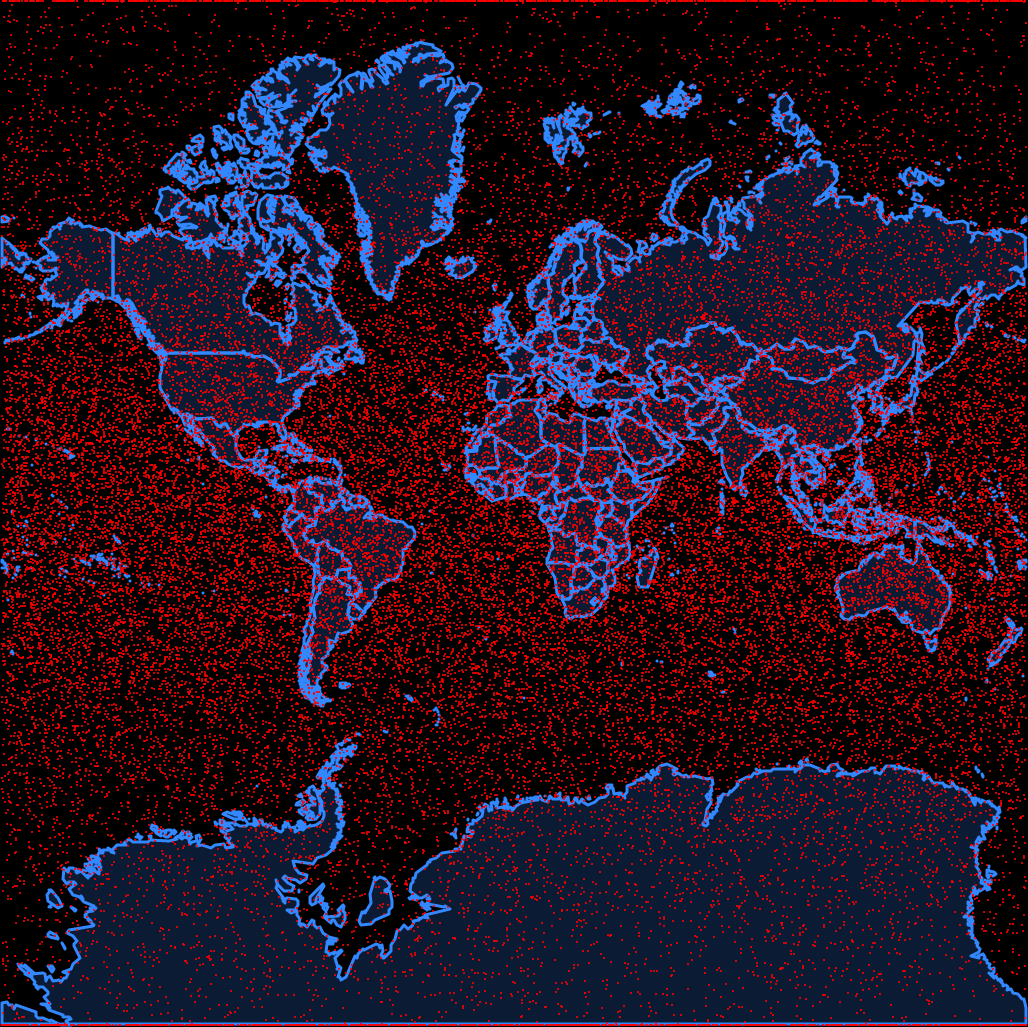
\includegraphics[width=\textwidth]{uniform/44692_0}
        \caption[The first of three purely random datasets with an element count of 44692.]{The first of three purely random datasets with an element count of 44692.}
        \label{sfig:uniform44692_0}
    \end{subfigure}\hfill
    \begin{subfigure}{0.4\textwidth}
        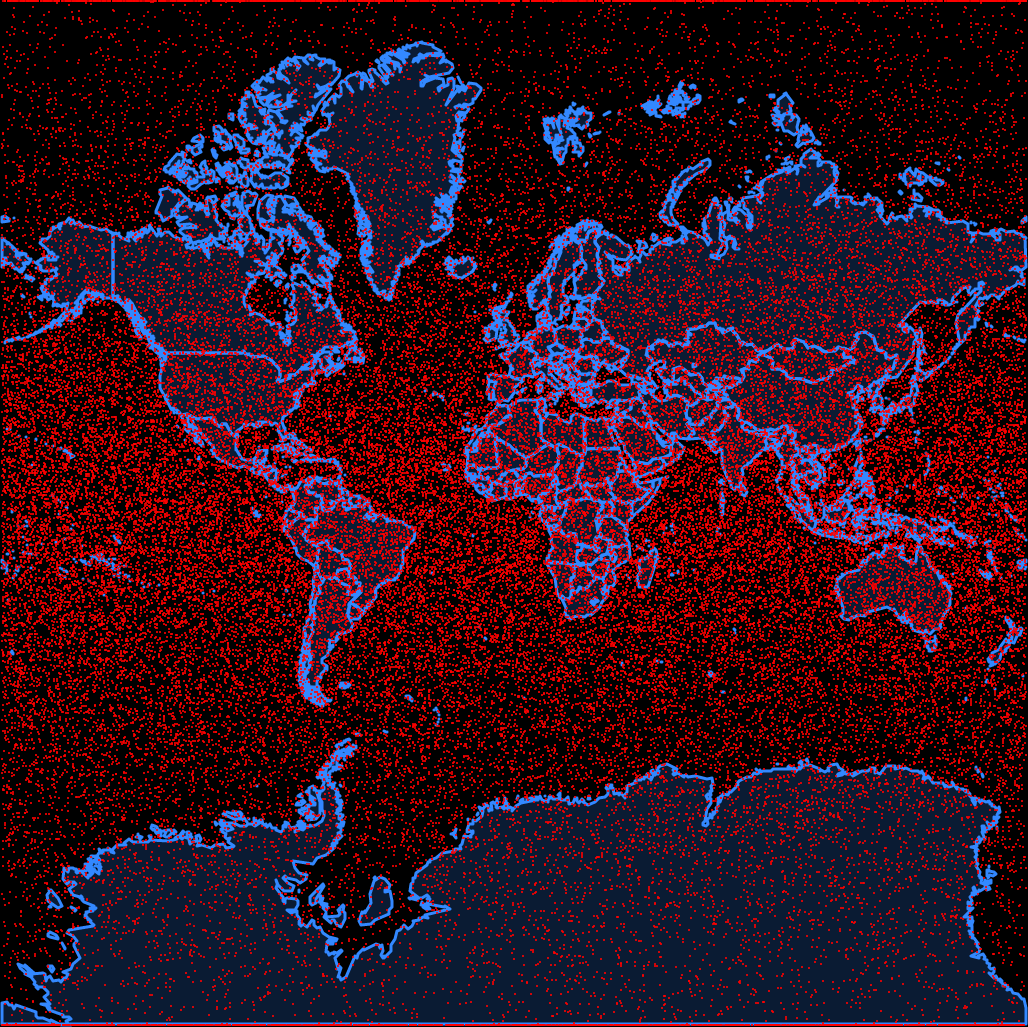
\includegraphics[width=\textwidth]{uniform/64800_0}
        \caption[The first of three purely random datasets with an element count of 64800.]{The first of three purely random datasets with an element count of 64800.}
        \label{sfig:uniform64800_0}
    \end{subfigure}\hfill
    \begin{subfigure}{0.4\textwidth}
        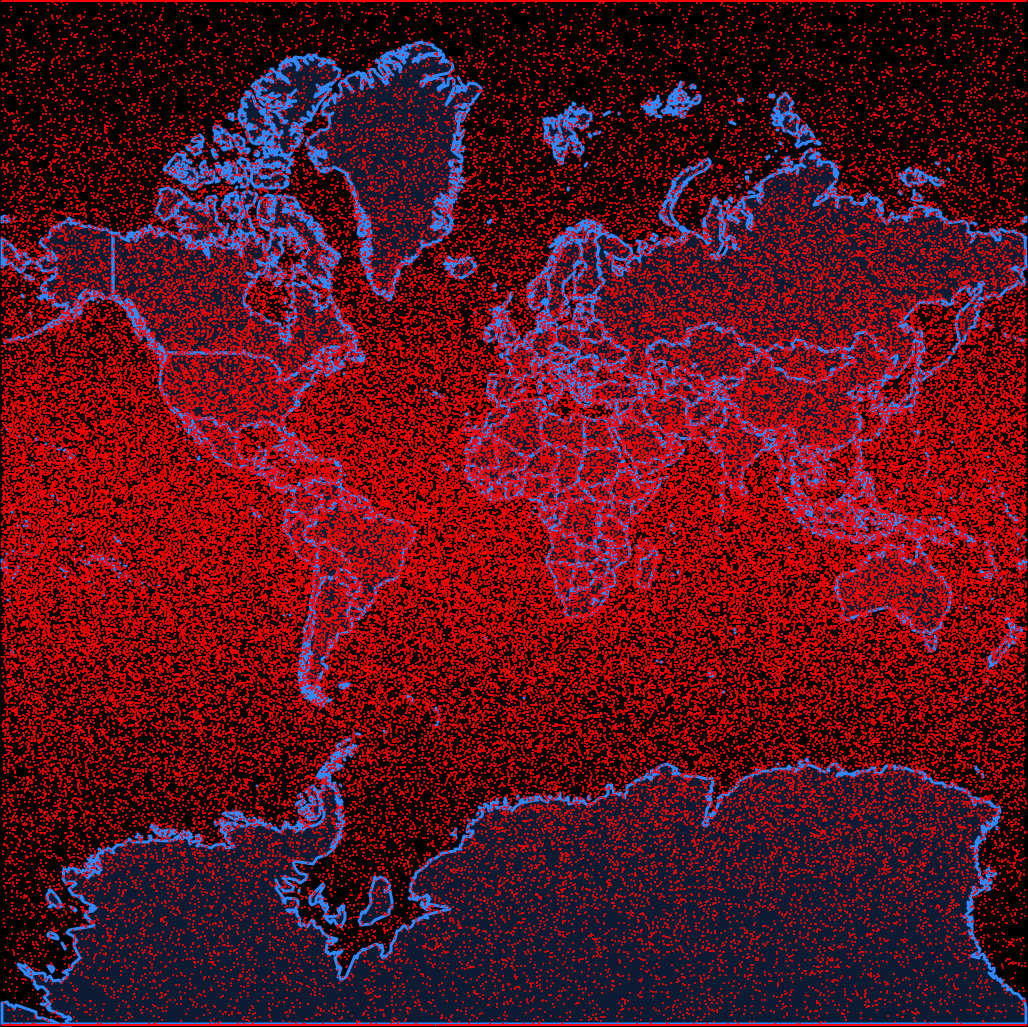
\includegraphics[width=\textwidth]{uniform/140974_0}
        \caption[The first of three purely random datasets with an element count of 140974.]{The first of three purely random datasets with an element count of 140974.}
        \label{sfig:uniform140974_0}
    \end{subfigure}\hfill
    \begin{subfigure}{0.4\textwidth}
        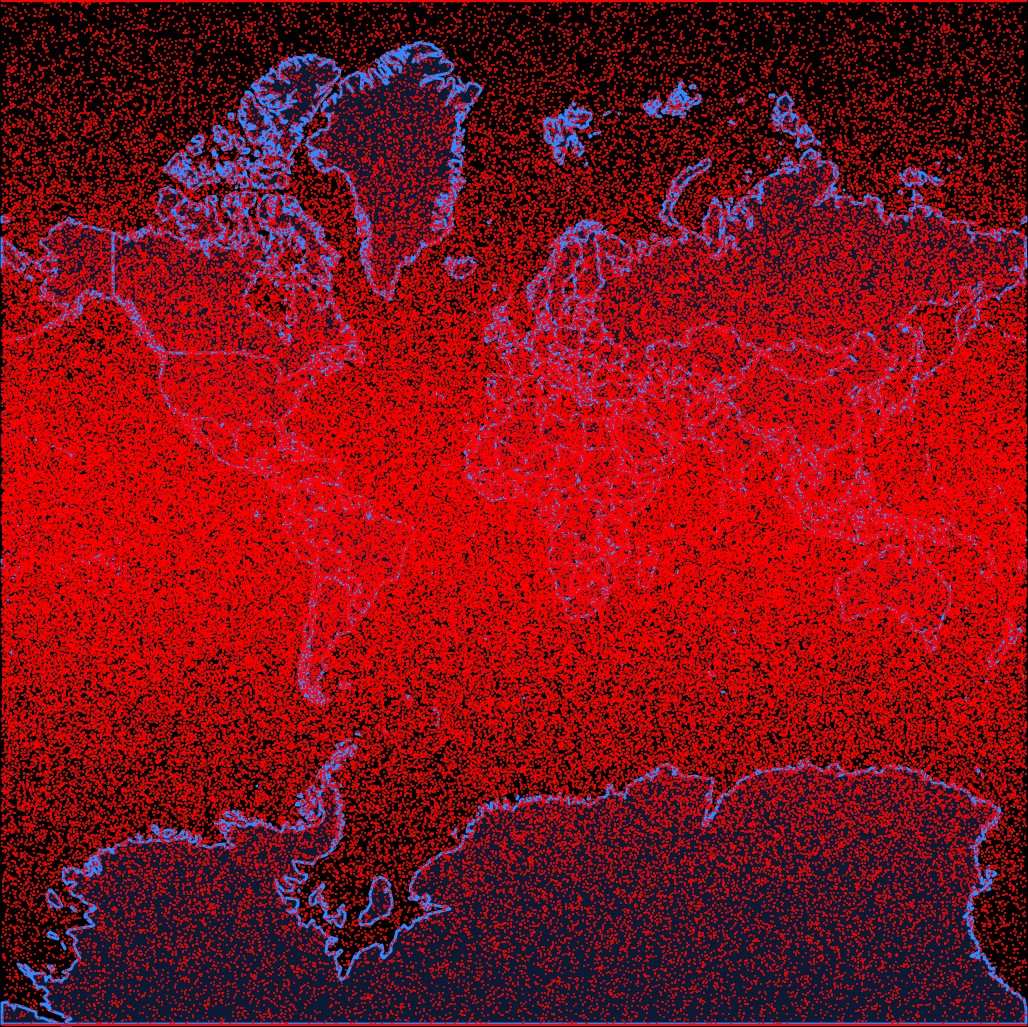
\includegraphics[width=\textwidth]{uniform/259200_0}
        \caption[The first of three purely random datasets with an element count of 259200.]{The first of three purely random datasets with an element count of 259200.}
        \label{sfig:uniform259200_0}
    \end{subfigure}\hfill
    \begin{subfigure}{0.4\textwidth}
        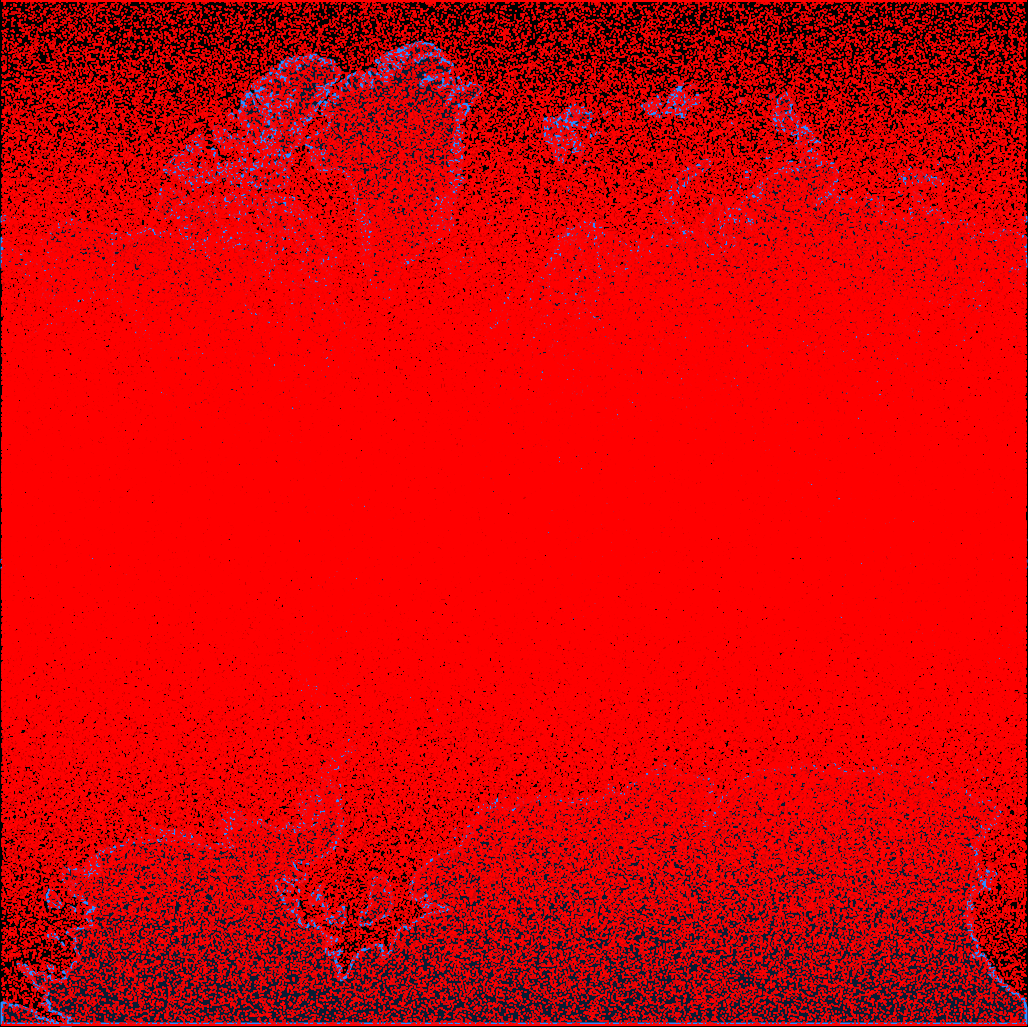
\includegraphics[width=\textwidth]{uniform/1036800_0}
        \caption[The first of three purely random datasets with an element count of 1036800.]{The first of three purely random datasets with an element count of 1036800.}
        \label{fig:uniform1036800_0}
    \end{subfigure}
    \caption[A selection of the random datasets.]{A selection of the random datasets.}
    \label{fig:uniform}
\end{figure}

\subsubsection{Synthetic - Randomly Clustered}
\label{subsubs:clustered}

The clustered dataset is constructed like the random dataset in \autoref{subsubs:random}, except that the points are generated in a radius around randomly generated points as to create distributed clusters of points. This is done to further test how distribution affects performance. This is closer to how elements are distributed in a real dataset when compared to a fully uniform distribution while still being easy to generate.

\begin{figure}[H]
    \centering
    \begin{subfigure}{0.458\textwidth}
        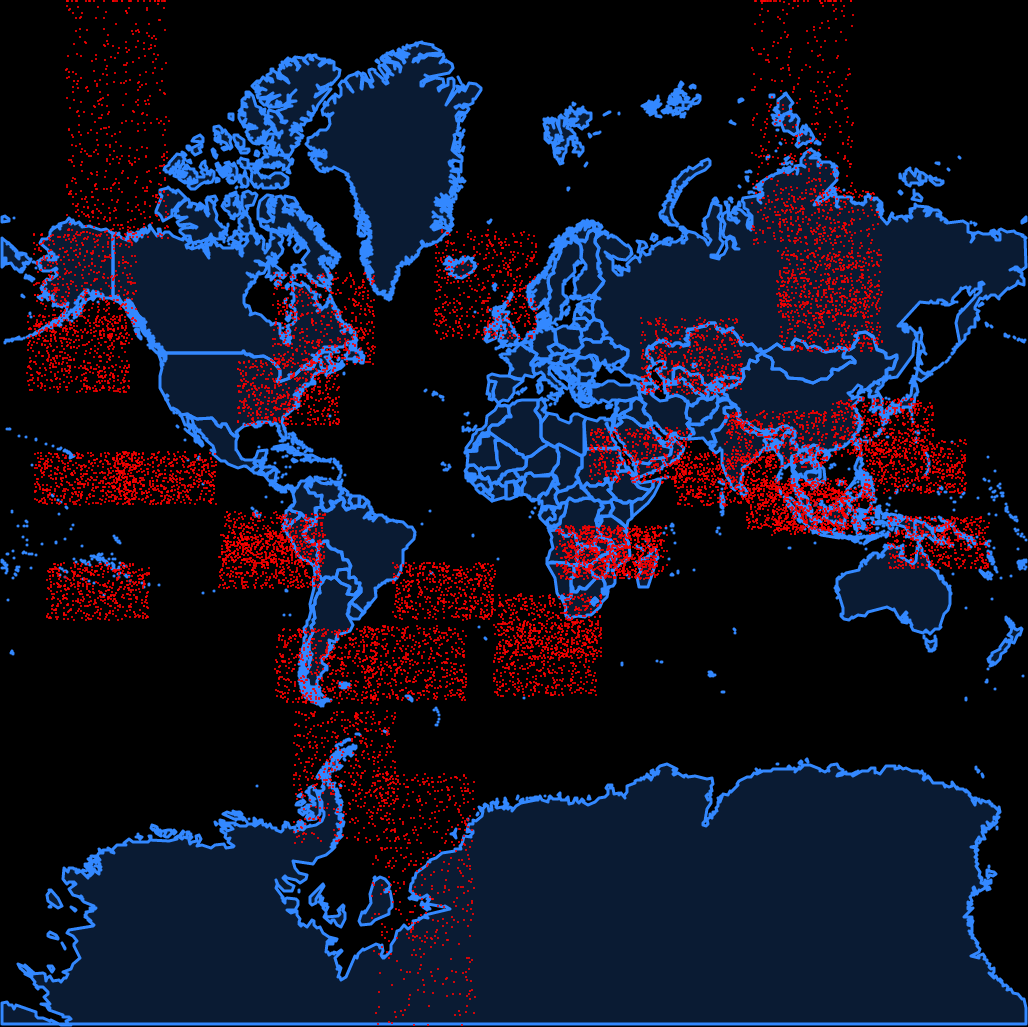
\includegraphics[width=\textwidth]{clustered/506_32_0}
        \caption[The first of three randomly clustered datasets to have 506 elements in 32 clusters.]{The first of three randomly clustered datasets to have 506 elements in 32 clusters.}
        \label{fig:clustered506_32_0}
    \end{subfigure}\hfill
    \begin{subfigure}{0.458\textwidth}
        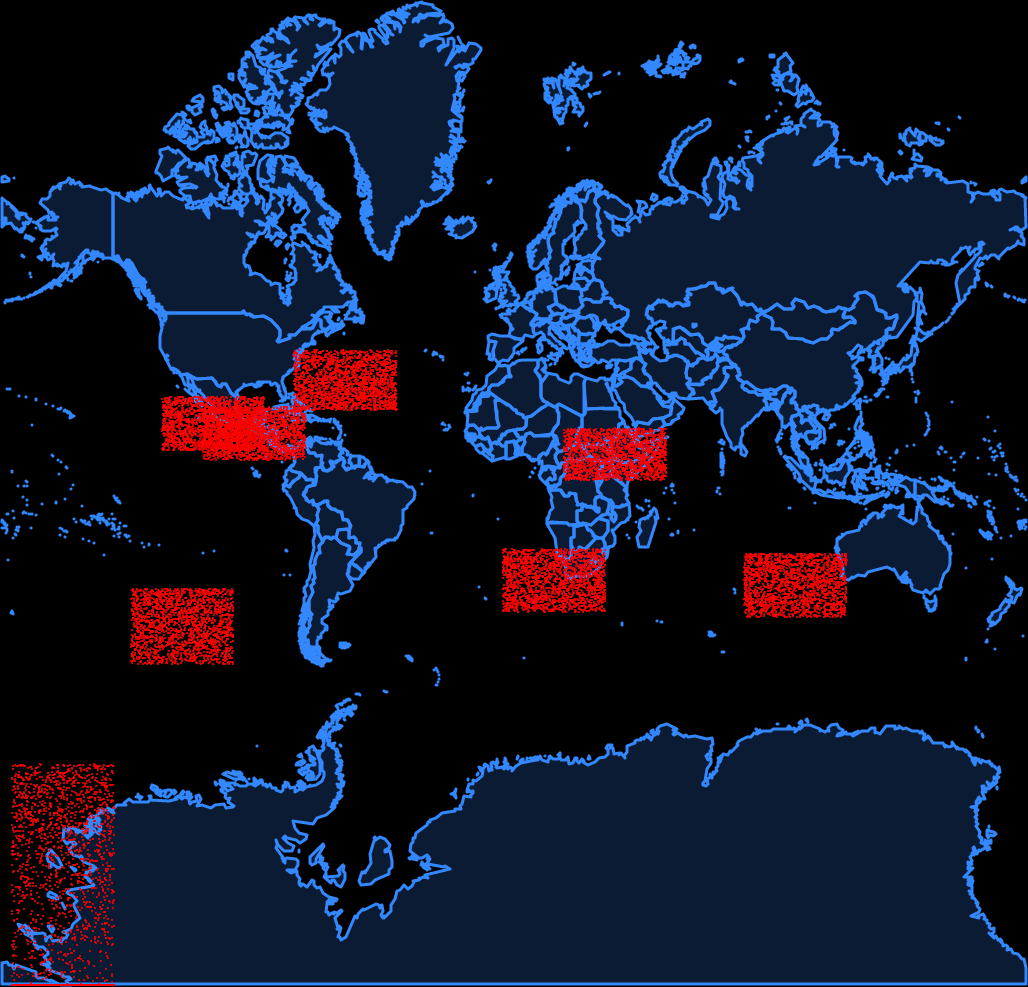
\includegraphics[width=\textwidth]{clustered/2025_8_0}
        \caption[The first of three randomly clustered datasets to have 2025 elements in 8 clusters.]{The first of three randomly clustered datasets to have 2025 elements in 8 clusters.}
        \label{fig:clustered2025_8_0}
    \end{subfigure}\hfill
    \begin{subfigure}{0.458\textwidth}
        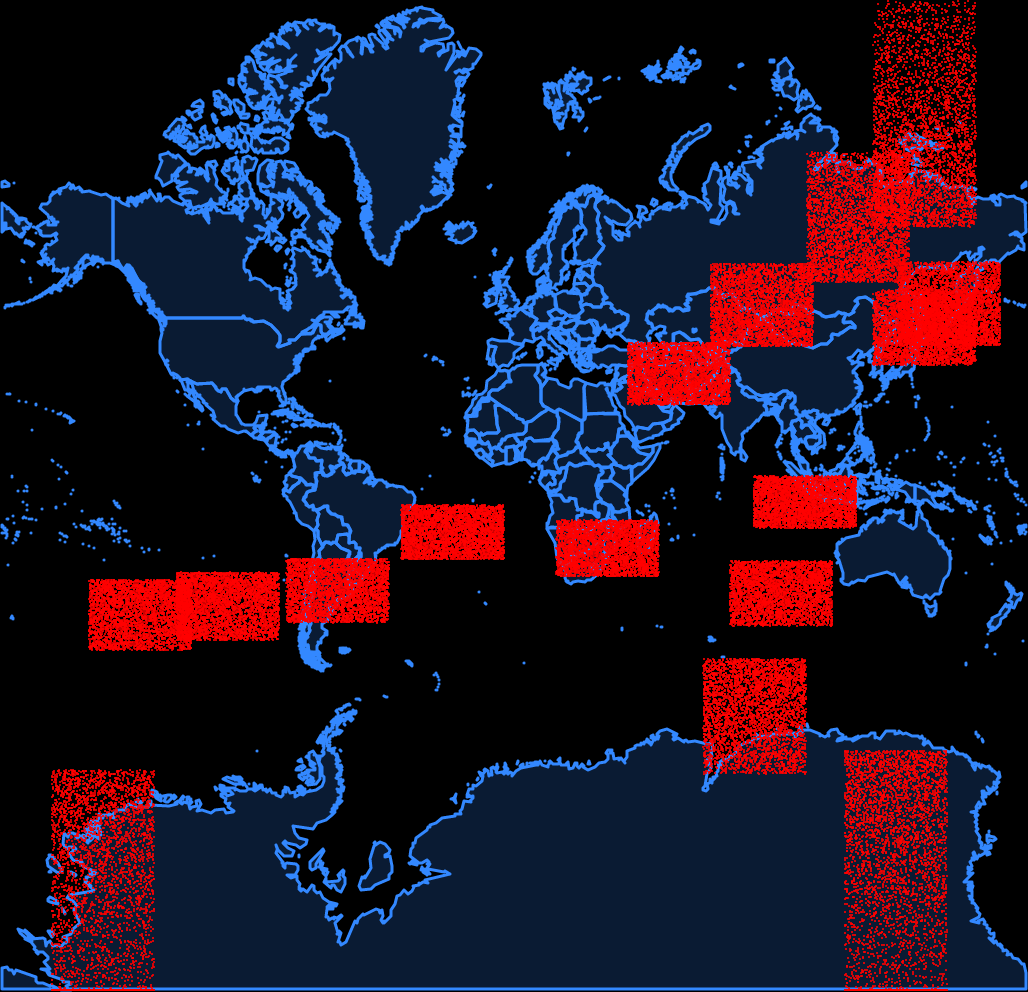
\includegraphics[width=\textwidth]{clustered/4050_16_2}
        \caption[The third of three randomly clustered datasets to have 4050 elements in 16 clusters.]{The third of three randomly clustered datasets to have 4050 elements in 16 clusters.}
        \label{fig:clustered4050_16_2}
    \end{subfigure}\hfill
    \begin{subfigure}{0.458\textwidth}
        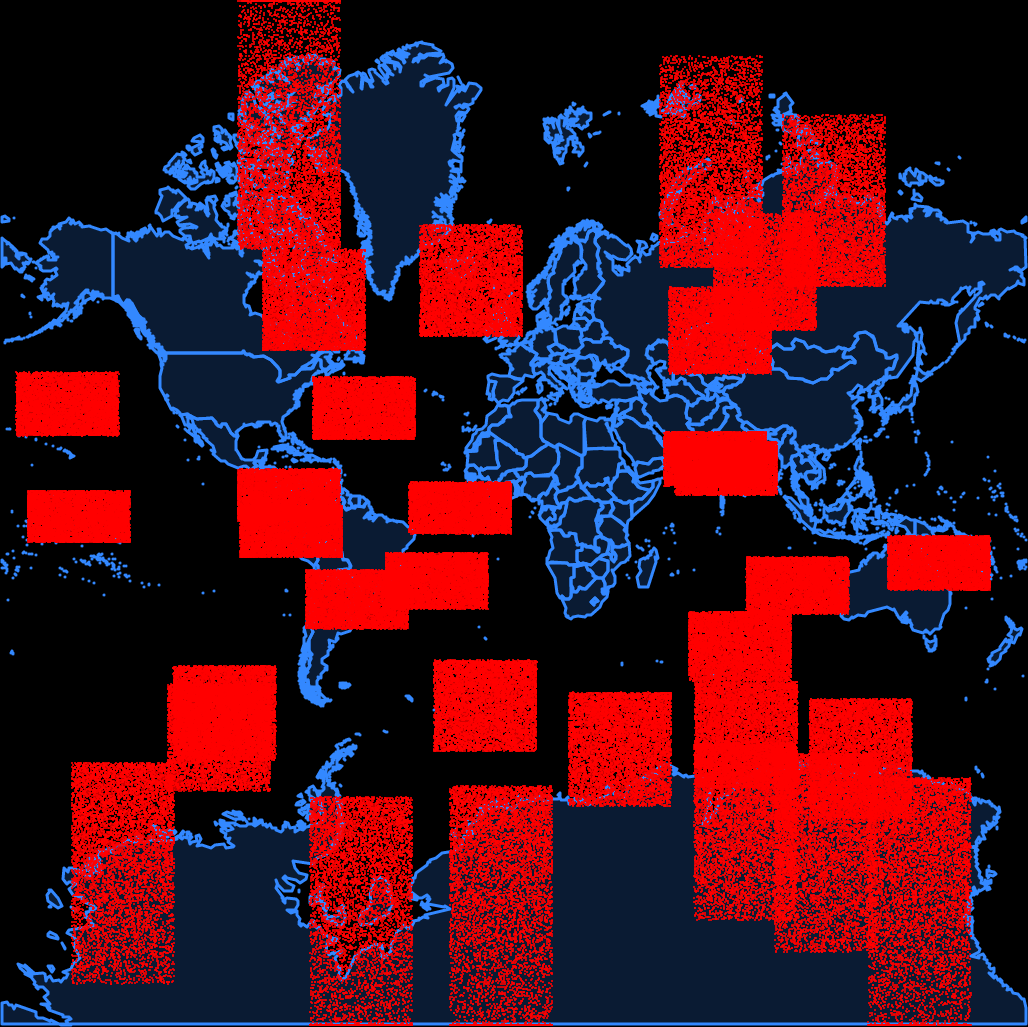
\includegraphics[width=\textwidth]{clustered/8100_32_0}
        \caption[The first of three randomly clustered datasets to have 8100 elements in 32 clusters.]{The third of three randomly clustered datasets to have 8100 elements in 32 clusters.}
        \label{fig:clustered8100_32_0}
    \end{subfigure}
    \caption[A selection of the randomly clustered datasets.]{A selection of the randomly clustered datasets.}
    \label{fig:clustered}
\end{figure}

\subsubsection{Real}

There are multiple different real datasets in use: The first\cite{simplemaps} and smallest consists of 44,692 points representing prominent cities. The second\cite{opendata} contains 140,974 cities and the third\cite{matthe} and final dataset incudes 4,384,909 points in theory - in practice, with invalid entries (such as missing coordinates) excluded, it still includes 3,808,651 entries.

\begin{figure}[H]
    \centering
    \begin{subfigure}{0.458\textwidth}
        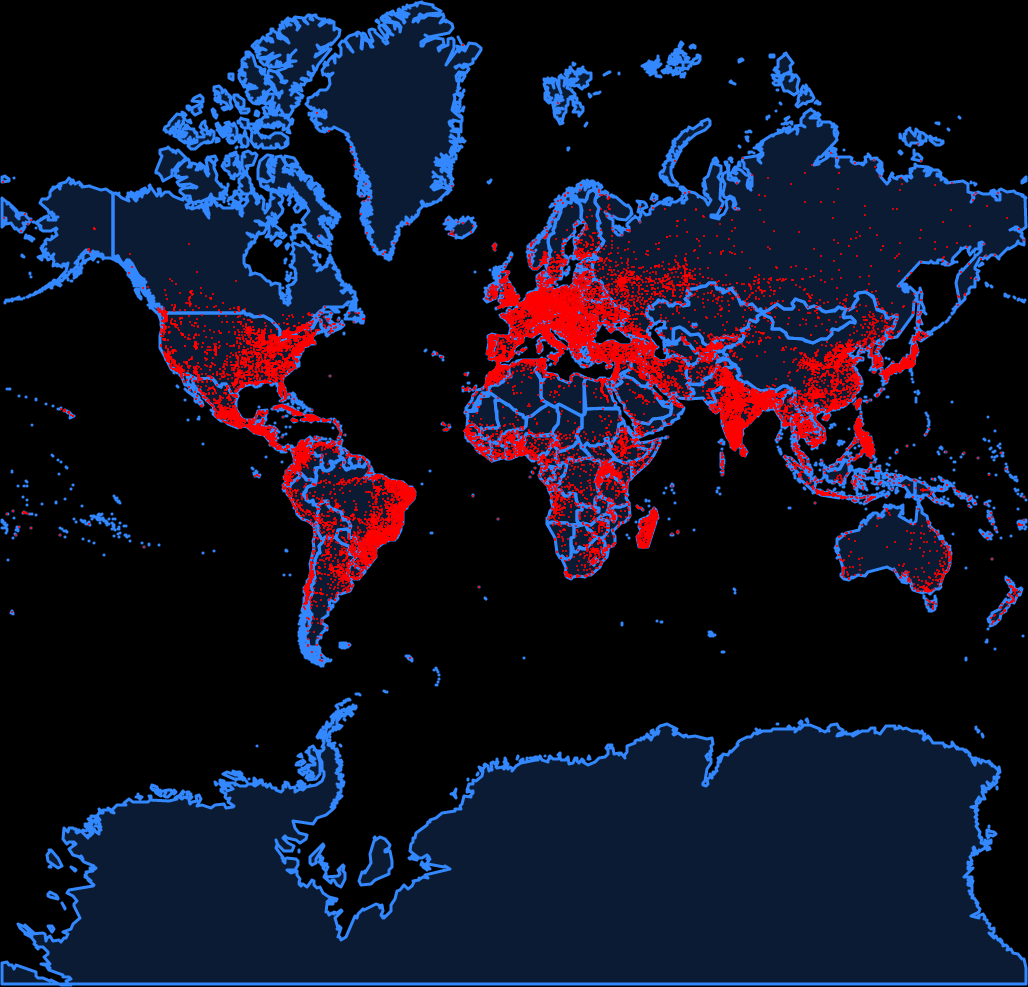
\includegraphics[width=\textwidth]{simple}
        \caption[The first of three real datasets (44,692 elements).]{The first of three real datasets (44,692 elements).}
        \label{fig:readsimple}
    \end{subfigure}
    \hfill
    \begin{subfigure}{0.458\textwidth}
        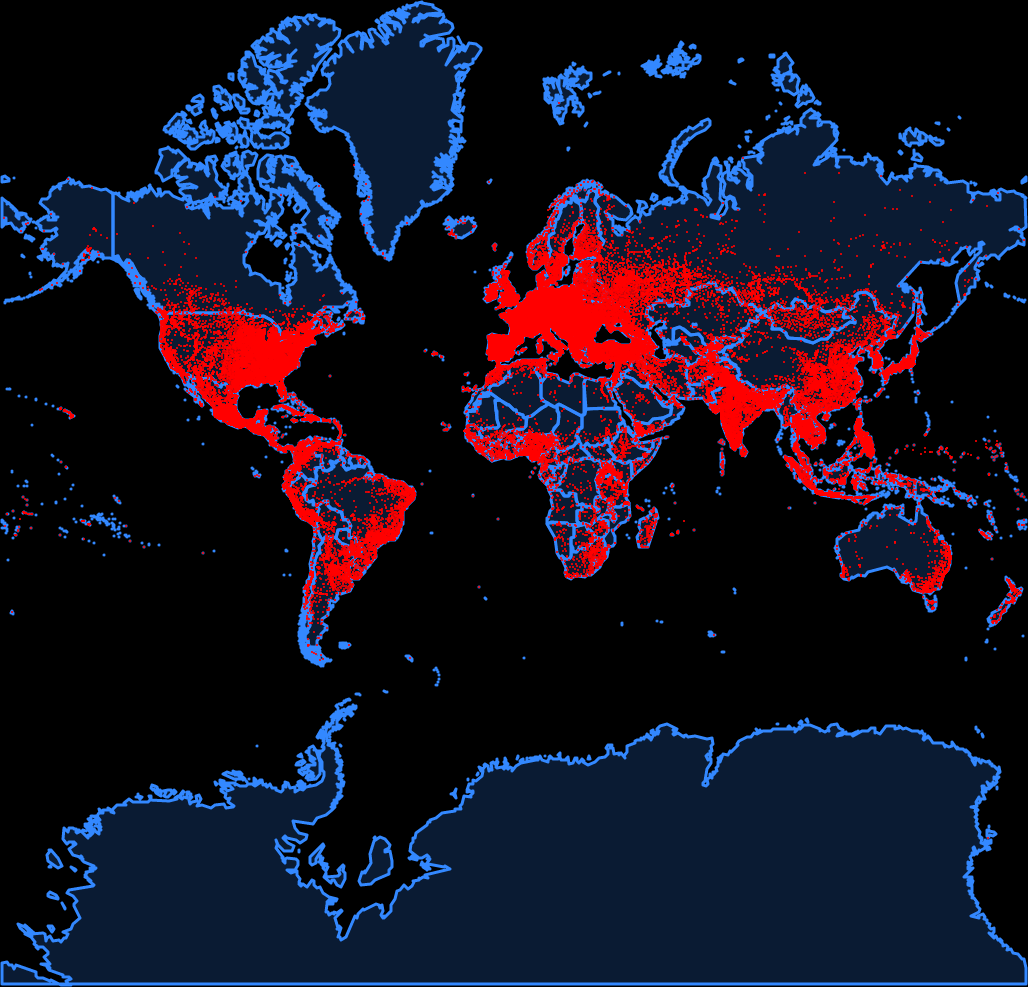
\includegraphics[width=\textwidth]{opendata}
        \caption[The second of three real datasets (140,974 elements).]{The second of three real datasets (140,974 elements).}
        \label{fig:realopen}
    \end{subfigure}
    \hfill
    \begin{subfigure}{0.458\textwidth}
        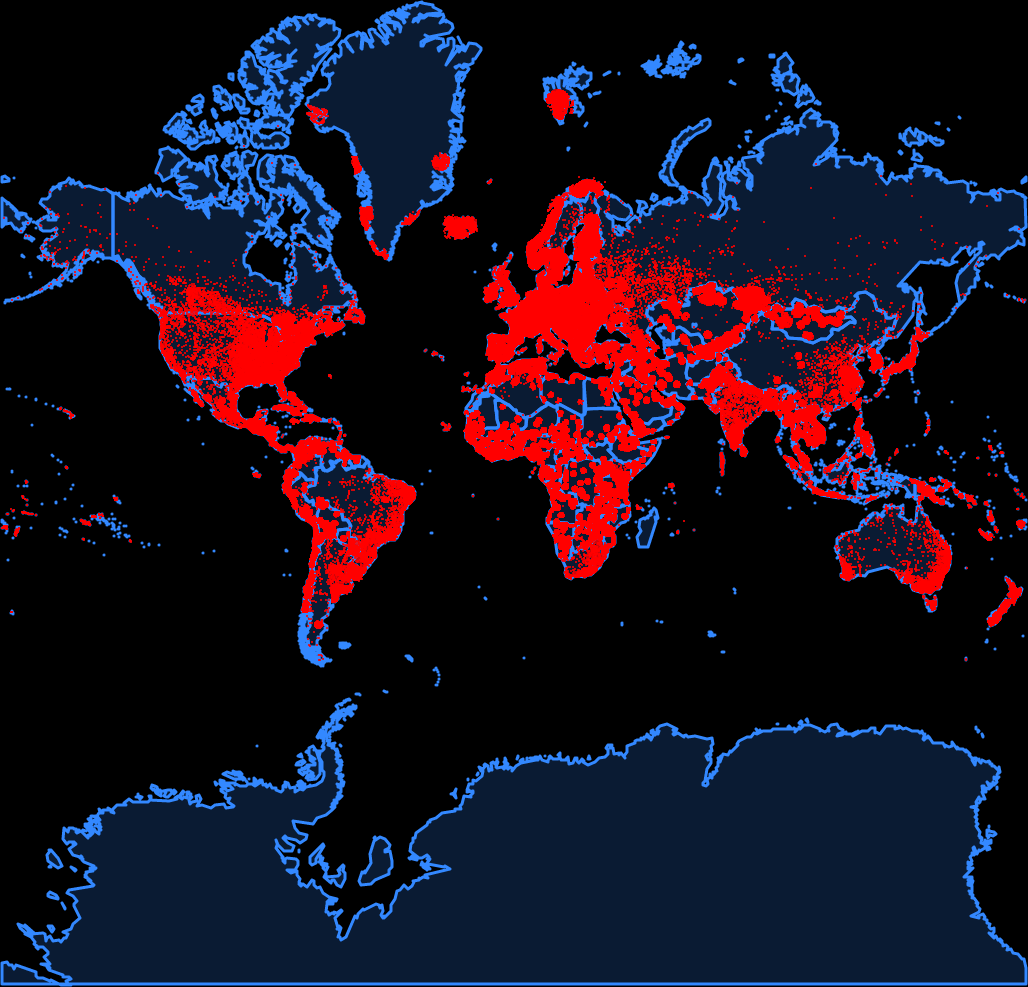
\includegraphics[width=\textwidth]{matthe}
        \caption[The third of three real datasets (4,384,909 elements).]{The third of three real datasets (4,384,909 elements).}
        \label{fig:realmatthe}
    \end{subfigure}
    \caption[All real datasets.]{All real datasets.}
    \label{fig:real}
\end{figure}

\section{Metrics}

Multiple metrics are used to compare the different datasets:

\subsection{Size in Memory}

While computers today do have a lot of memory by comparison, the memory requirements for nearly everything have grown quite a bit as well and so have the available / necessary datasets. In addition to this, the smaller something is in memory, the faster it can be iterated through - a smaller memory footprint is always an advantage.\\
This metric measures the sum of all allocations for each data structure. It does not take memory layout into account. It also does not count over-allocation\footnote{While allocator \acsp{API} generally allow to request an arbitrary number of bytes, most do not guarantee that the returned memory block is exactly the requested size - only that it is at least as big. This can be for several reasons: To work against fragmentation, to store additional information about the allocation or to make future in-place growing of the allocation possible.}. So a single allocation of 1MiB would count the same as 1024 allocations that request 1 byte each, even though (in reality) the latter would most likely use up more memory and cause heap fragmentation.

\subsection{Time to Build}

Being able to build a data structure faster enables a higher update frequency for internally immutable data structures. A higher update frequency means more current information being exposed through the index. When optimising for read performance, using internally immutable data structures makes sense as this removes the need for synchronisation, fencing and similar mechanisms (which hurt performance to be able to guarantee deterministic / safe behaviour) when utilising parallelisation and/or asynchronicity. The latter, again, just makes sense when optimising for performance - which is probably why one of these indices would be used in the first place.\\
This metric measures the time it takes for the structure to load the data and to modify that data so that efficient querying is possible. To improve comparability, the dataset is always preloaded into memory first - which is not measured. This way \acs{I/O} performance (which can be quite flakey) is cut out of the equation. To make sure that all of the data was actually loaded, the number of elements in the index is compared with the number of entries in the source dataset - this is also not measured.

\subsection{Time to Delete}

Being able to delete a data structure faster means that the previously allocated memory is made available to be allocated again more quickly. This can help to keep the average memory consumption of a process down. Deletions, or rather deallocations, are constant-time actions, generally. However, if a data structure allocates multiple times, even more so if it does so recursively, it also needs to deallocate multiple times - so the more allocations, the more deallocations, the longer deletion takes. This is even worse if pointer-chasing\footnote{When data can only be reached through a series of pointers, where one points to the next. This is generally necessary for dynamically sized data structures that are not stored in a contiguous block of memory - through to different degrees, based on the data structure.} is necessary, like with linked lists, or even more so with tree-like structures where a node owns multiple other nodes recursively.\\
To get this metric, the previously built data structure is manually deallocated - the execution time of this deallocation function is measured.

\subsection{Time to Query}

Querying is the core functionality of indices, all preparation beforehand is done so that querying can be as efficient as possible. Faster queries simply means that more queries can be done per second - so to achieve a higher throughput (unless there is a bottleneck somewhere else - which in a networked environment, like with a server, is quite likely).\\
This metric is not as straight forward to measure as the others, there are infinitely many possible queries for each dataset (if we had infinite precision arithmetic that is). So there is only one option: Picking a subset of queries that share significant parameters. For this purpose two kinds of queries will be used:

\subsubsection{Query All}

For the \textit{query all} benchmark, a given index is simply asked to return all points in its extent. This has one obvious flaw: It is dependent on the size of the index. When comparing an index with one that is twice as big, the latter has to do at the very least twice as much work just moving the data. So comparing this is mostly useful for indices with the same raw amount of data. Otherwise the resulting number could potentially be given relative to the ratio between the sizes of the two datasets.

\subsubsection{Prepared Queries}

The idea behind the prepared queries is as follows: It should be possible to randomly generate a set of \acsp{BBox} for every dataset so that each one contains \textit{n} elements. This is then done 16 times for every \(n \in \{16, 64, 256, 1024, 4096\}\). Now it is possible to go through every dataset and measure how long it takes to retrieve \textit{n} elements and analyse, how the element size and count affect this and how well the different indices handle it for each of the element distributions.

\section{Compared Libraries}

At this stage two libraries are included in this comparison:

\paragraph{rstar} The first library implements an \textit{R*Tree}, it is found on \textit{Rust's} package index under the following url: \url{https://crates.io/crates/rstar} at version \textit{0.11.0}.

\paragraph{hprtree} The other library implements an \acs{HPRTree}, it is found on \textit{Rust's} package index under the following url: \url{https://crates.io/crates/hprtree} at commit \textit{df396bd7090a8370\-78aafac2b5a0cec575872df6} of the master branch (one commit after version \textit{0.2.2}).


\section{General Considerations}
\label{sec:considerations}

A few general considerations are necessary before the benchmarking can commence:

\paragraph{Priority} As processes running on multitasking operating systems share (and thus compete) for the same resources, they affect each others performance. Because of this, the process priority of the benchmarking process is set to the maximum available (24 - \textit{Real Time}) on the Windows operating system. While \acs{I/O}-operations are intentionally excluded from the benchmarks having a lower \acs{I/O} priority should not matter. Still this one is also set to the maximum available (in this case \textit{High}).

\paragraph{Swapping} Another variable that can affect performance is swapping (also called paging): Computers tend to be allowed to move \acs{RAM} content to disk. This is great because it provides the computer a lot of capacity, however this is also bad because this can cause hard (sometimes also called major) page faults. This happens if a program attempts to access a section of memory that is not currently located in \acs{RAM} - when this happens the operating system has to load that piece of memory in the the resulting fault handler, which results in a lot of (potentially inconsistent) latency as the memory access has essentially become an \acs{I/O}-operation. Sometimes the operating system might also have to page another section of memory out, before it can page the requested section in, which makes the aforementioned effects even worse. For these reasons, swapping is disabled on the machine carrying out the benchmarks. This also means that if a datastructure attempts to allocate more memory than is physically available, it will fail to allocate - in many environments this is an unrecoverable error (the only exceptions the author can think of are the kernel finding and killing other processes that use up sufficient memory in the fault handler or a memory-managed environment like the \acs{JVM} attempting to compact the heap).